%-----------------------------------------------------------------------
% Usar opção handout para disponibilizar slides
\documentclass[handout,serif, professionalfont, usenames, dvipsnames, aspectratio = 169]{beamer}\usepackage[]{graphicx}\usepackage[]{color}
% maxwidth is the original width if it is less than linewidth
% otherwise use linewidth (to make sure the graphics do not exceed the margin)
\makeatletter
\def\maxwidth{ %
  \ifdim\Gin@nat@width>\linewidth
    \linewidth
  \else
    \Gin@nat@width
  \fi
}
\makeatother

\definecolor{fgcolor}{rgb}{0.396, 0.482, 0.514}
\newcommand{\hlnum}[1]{\textcolor[rgb]{0.863,0.196,0.184}{#1}}%
\newcommand{\hlstr}[1]{\textcolor[rgb]{0.863,0.196,0.184}{#1}}%
\newcommand{\hlcom}[1]{\textcolor[rgb]{0.576,0.631,0.631}{#1}}%
\newcommand{\hlopt}[1]{\textcolor[rgb]{0.345,0.431,0.459}{#1}}%
\newcommand{\hlstd}[1]{\textcolor[rgb]{0.396,0.482,0.514}{#1}}%
\newcommand{\hlkwa}[1]{\textcolor[rgb]{0.796,0.294,0.086}{#1}}%
\newcommand{\hlkwb}[1]{\textcolor[rgb]{0.522,0.6,0}{#1}}%
\newcommand{\hlkwc}[1]{\textcolor[rgb]{0.796,0.294,0.086}{#1}}%
\newcommand{\hlkwd}[1]{\textcolor[rgb]{0.345,0.431,0.459}{#1}}%
\let\hlipl\hlkwb

\usepackage{framed}
\makeatletter
\newenvironment{kframe}{%
 \def\at@end@of@kframe{}%
 \ifinner\ifhmode%
  \def\at@end@of@kframe{\end{minipage}}%
  \begin{minipage}{\columnwidth}%
 \fi\fi%
 \def\FrameCommand##1{\hskip\@totalleftmargin \hskip-\fboxsep
 \colorbox{shadecolor}{##1}\hskip-\fboxsep
     % There is no \\@totalrightmargin, so:
     \hskip-\linewidth \hskip-\@totalleftmargin \hskip\columnwidth}%
 \MakeFramed {\advance\hsize-\width
   \@totalleftmargin\z@ \linewidth\hsize
   \@setminipage}}%
 {\par\unskip\endMakeFramed%
 \at@end@of@kframe}
\makeatother

\definecolor{shadecolor}{rgb}{.97, .97, .97}
\definecolor{messagecolor}{rgb}{0, 0, 0}
\definecolor{warningcolor}{rgb}{1, 0, 1}
\definecolor{errorcolor}{rgb}{1, 0, 0}
\newenvironment{knitrout}{}{} % an empty environment to be redefined in TeX

\usepackage{alltt}
%\documentclass[serif, professionalfont, usenames, dvipsnames, aspectratio = 169]{beamer}
\usepackage[T1]{fontenc}

% \usetheme{Copenhagen}

% Definição do esquema de cores:
% 1. UFPR - Azul com cinza.
% 2. DEST - Roxo com cinza.
% 3. LEG - Laranjado com cinza.
\def\mycolorscheme{1}

% Caminho para a imagem de fundo com aspecto 16x9.
% \def\pathtobg{config/ufpr-fachada-baixo-1.jpg}
% \def\pathtobg{config/ufpr-fundo.jpg}
% \def\pathtobg{config/ufpr-fundo.jpg}
\def\pathtobg{config/ufpr-fundo-16x9.jpg}

% ATTENTION: preamble.tex contains all style definitions.
%-----------------------------------------------------------------------

% Palladio.
% \usepackage[sc]{mathpazo}
% \linespread{1.05}         % Palladio needs more leading (space between lines)
% \usepackage[T1]{fontenc}

% Kurier.
% \usepackage[light, condensed, math]{kurier}
% \usepackage[T1]{fontenc}

% Iwona.
% \usepackage[math, light, condensed]{iwona}

% \usepackage{cmbright}
% \usepackage[charter]{mathdesign}
% \usepackage{palatino}

% Roboto (with Iwona for maths).
% \usepackage[math]{iwona}
% \usepackage[sfdefault, light, condensed]{roboto}

% Source Sans Pro (with Iwona for maths).
% \usepackage[math]{iwona}
% \usepackage[default, light]{sourcesanspro}

% Lato (with Iwona for maths).
% \usepackage[math]{iwona}
% \usepackage[default]{lato}

% Fira Sans (with Iwona for maths).
\usepackage[math, light]{iwona}
\usepackage[sfdefault,light]{FiraSans} %% option 'sfdefault' activates Fira Sans as the default text font
\usepackage[T1]{fontenc}
\renewcommand*\oldstylenums[1]{{\firaoldstyle #1}}

% Font for code. ----------------------------
% \usepackage[scaled=.75]{beramono}
\usepackage{inconsolata}

\usepackage{amstext} % for \text macro
\usepackage{array}   % for \newcolumntype macro
\newcolumntype{L}{>{$}l<{$}} % math-mode version of "l" column type

% ATTENTION: needs complile with xelatex: `$ xelatex file.tex`
% \usepackage{fontspec}
% \setmonofont{M+ 1m}
% \setmonofont{M+ 1mn}
% \setmonofont{M+ 2m}

%-----------------------------------------------------------------------

% \usepackage{lmodern}
\usepackage{amssymb, amsmath}
\usepackage[makeroom]{cancel}
% \usepackage{ifxetex, ifluatex}
\usepackage{fixltx2e} % provides \textsubscript
\usepackage[utf8]{inputenc}
\usepackage[shorthands=off,main=brazil]{babel}
\usepackage{graphicx}
\usepackage{color}
\usepackage{xcolor}
\usepackage{setspace}
\usepackage{comment}
\usepackage{icomma}

%-----------------------------------------------------------------------
% Algumas configurações.

\setlength{\parindent}{0pt}
\setlength{\parskip}{6pt plus 2pt minus 1pt}
\setlength{\emergencystretch}{3em}  % prevent overfull lines
% \providecommand{\tightlist}{%
%   \setlength{\itemsep}{0pt}\setlength{\parskip}{0pt}}
\setcounter{secnumdepth}{0}

% Espaço vertical para o ambiente `quote`.
\let\oldquote\quote
\let\oldendquote\endquote
\renewenvironment{quote}{%
  \vspace{1em}\oldquote}{%
  \oldendquote\vspace{1em}}

%-----------------------------------------------------------------------
% Espaçamento entre items para itemize, enumerate e description.

% % itemize.
% \let\itemopen\itemize
% \let\itemclose\enditemize
% \renewenvironment{itemize}{%
%   \itemopen\addtolength{\itemsep}{0.25\baselineskip}}{\itemclose}
%
% % enumerate.
% \let\enumopen\enumerate
% \let\enumclose\endenumerate
% \renewenvironment{enumerate}{%
%   \enumopen\addtolength{\itemsep}{0.25\baselineskip}}{\enumclose}
%
% % description.
% \let\descopen\description
% \let\descclose\enddescription
% \renewenvironment{description}{%
%   \descopen\addtolength{\itemsep}{0.25\baselineskip}}{\descclose}

%-----------------------------------------------------------------------

% \usepackage[hang]{caption}
\usepackage{caption}
\captionsetup{font=footnotesize,
  labelfont={color=mycolor1, footnotesize},
  labelsep=period}

% \providecommand{\tightlist}{%
%   \setlength{\itemsep}{0pt}\setlength{\parskip}{0pt}}

%-----------------------------------------------------------------------

\usepackage{tikz}

% \def\pathtobg{/home/walmes/Projects/templates/COMMON/ufpr-fundo.jpg}
% \def\pathtobg{/home/walmes/Projects/templates/COMMON/ufpr-fundo-16x9.jpg}
% \def\pathtobg{/home/walmes/Projects/templates/COMMON/ufpr-fachada-dir-1.jpg}
% \def\pathtobg{/home/walmes/Projects/templates/COMMON/ufpr-fachada-esq-1.jpg}
% \def\pathtobg{/home/walmes/Projects/templates/COMMON/ufpr-perto-1.jpg}
% \def\pathtobg{/home/walmes/Projects/templates/COMMON/ufpr-fachada-baixo-1.jpg}

\ifx\pathtobg\undefined
\else
  \usebackgroundtemplate{
    \tikz[overlay, remember picture]
    \node[% opacity=0.3,
          at=(current page.south east),
          anchor=south east,
          inner sep=0pt] {
            \includegraphics[height=\paperheight, width=\paperwidth]{\pathtobg}};
  }
\fi

%-----------------------------------------------------------------------
% Definições de esquema de cores.

\ifx\mycolorscheme\undefined
  % UFPR.
  % http://www.color-hex.com/color-palette/2018
  \definecolor{mycolor1}{HTML}{015c93} % Título.
  \definecolor{mycolor2}{HTML}{363435} % Texto.
  \definecolor{mycolor3}{HTML}{015c93} % Estrutura.
  \definecolor{mycolor4}{HTML}{015c93} % Links.
  \definecolor{mycolor5}{HTML}{CECAC5} % Preenchimentos.
\else
  \if\mycolorscheme1
    % UFPR.
    \definecolor{mycolor1}{HTML}{015c93} % Título.
    \definecolor{mycolor2}{HTML}{363435} % Texto.
    \definecolor{mycolor3}{HTML}{015c93} % Estrutura.
    \definecolor{mycolor4}{HTML}{015c93} % Links.
    \definecolor{mycolor5}{HTML}{CECAC5} % Preenchimentos.
  \fi
  \if\mycolorscheme2
    % DEST.
    \definecolor{mycolor1}{HTML}{2a0e72} % Título.
    \definecolor{mycolor2}{HTML}{202E35} % Texto.
    \definecolor{mycolor3}{HTML}{2a0e72} % Estrutura.
    % \definecolor{mycolor3}{HTML}{8072a3} % Estrutura.
    \definecolor{mycolor4}{HTML}{2a0e72} % Links.
    % \definecolor{mycolor4}{HTML}{bfb9d1} % Links.
    % \definecolor{mycolor5}{HTML}{AEA79F} % Preenchimentos.
    \definecolor{mycolor5}{HTML}{CECAC5} % Preenchimentos.
  \fi
  \if\mycolorscheme3
    % LEG.
    \definecolor{mycolor2}{HTML}{363435} % Texto.
    % \definecolor{mycolor1}{HTML}{ff8000} % Título.
    % \definecolor{mycolor3}{HTML}{ff8000} % Estrutura.
    % \definecolor{mycolor4}{HTML}{ff8000} % Links.
    % \definecolor{mycolor1}{HTML}{E57300} % Título.
    % \definecolor{mycolor3}{HTML}{E57300} % Estrutura.
    % \definecolor{mycolor4}{HTML}{E57300} % Links.
    \definecolor{mycolor1}{HTML}{F67014} % Título.
    \definecolor{mycolor3}{HTML}{F67014} % Estrutura.
    \definecolor{mycolor4}{HTML}{F67014} % Links.
    % \definecolor{mycolor1}{HTML}{FE5C23} % Título.
    % \definecolor{mycolor3}{HTML}{FE5C23} % Estrutura.
    % \definecolor{mycolor4}{HTML}{FE5C23} % Links.
    \definecolor{mycolor5}{HTML}{222222} % Preenchimentos.
    \definecolor{mycolor5}{HTML}{383838} % Preenchimentos.
  \fi
\fi

\hypersetup{
  colorlinks=true,
  linkcolor=mycolor4,
  urlcolor=mycolor1,
  citecolor=mycolor1
}

%-----------------------------------------------------------------------
% ATTENTION: http://www.cpt.univ-mrs.fr/~masson/latex/Beamer-appearance-cheat-sheet.pdf

\usetheme{Boadilla}
\usecolortheme{default}

% \setbeamersize{text margin left=7mm, text margin right=7mm}
% \setbeamertemplate{frametitle}[default][left, leftskip=3mm]
% \addtobeamertemplate{frametitle}{\vspace{0.5em}}{}

\setbeamertemplate{caption}[numbered]
\setbeamertemplate{section in toc}[sections numbered]
\setbeamertemplate{subsection in toc}[subsections numbered]
\setbeamertemplate{sections/subsections in toc}[ball]{}
\setbeamertemplate{sections in toc}[ball]
\setbeamercolor{section number projected}{bg=mycolor1, fg=white}
\setbeamertemplate{blocks}[rounded]
\setbeamertemplate{navigation symbols}{}
\setbeamertemplate{frametitle continuation}{\gdef\beamer@frametitle{}}
% \setbeamertemplate{frametitle}[default][center]
% \setbeamertemplate{footline}[frame number]

\setbeamertemplate{enumerate items}[default]
\setbeamertemplate{itemize items}{\scriptsize\raise1.25pt\hbox{\donotcoloroutermaths$\blacktriangleright$}}

% Blocos.
% \addtobeamertemplate{block begin}{\vskip -\bigskipamount}{}
% \addtobeamertemplate{block end}{}{\vskip -\bigskipamount}
\addtobeamertemplate{block begin}{\vspace{0.5em}}{}
\addtobeamertemplate{block end}{}{\vspace{0.5em}}


% Rodapé.
\setbeamercolor{title in head/foot}{parent=subsection in head/foot}
\setbeamercolor{author in head/foot}{bg=mycolor4, fg=white}
\setbeamercolor{date in head/foot}{parent=subsection in head/foot, fg=mycolor3}

% Cabeçalho.
\setbeamercolor{section in head/foot}{bg=mycolor2, fg=mycolor4}
\setbeamercolor{subsection in head/foot}{bg=mycolor2, fg=white}

\setbeamercolor{title}{fg=mycolor1}       % Título dos slides.
\setbeamercolor{titlelike}{fg=title}
\setbeamercolor{subtitle}{fg=mycolor2}    % Subtítulo.
\setbeamercolor{institute in head/foot}{parent=palette primary} % Instituição.
\setbeamercolor{frametitle}{fg=mycolor1}  % De quadro.
\setbeamercolor{structure}{fg=mycolor3}   % Listas e rodapé.
\setbeamercolor{item projected}{bg=mycolor2}
\setbeamercolor{block title}{bg=mycolor5, fg=mycolor2}
\setbeamercolor{normal text}{fg=mycolor2} % Texto.
\setbeamercolor{caption name}{fg=normal text.fg}
% \setbeamercolor{footlinecolor}{fg=mycolor2, bg=mycolor5}
% \setbeamercolor{section in head/foot}{fg=mycolor2, bg=mycolor5}
\setbeamercolor{author in head/foot}{fg=white, bg=mycolor1}
\setbeamercolor{section in foot}{fg=mycolor4, bg=mycolor5}
\setbeamercolor{date in foot}{fg=mycolor4, bg=mycolor5}
\setbeamercolor{block title}{fg=white, bg=mycolor1}
\setbeamercolor{block body}{fg=black, bg=white!80!gray}
\setbeamercolor{block body}{fg=black, bg=white!80!gray}

% To remove empty brackets of \institution.
\makeatletter
\setbeamertemplate{footline}{
  \leavevmode%
  \hbox{%
    \begin{beamercolorbox}[
      wd=0.3\paperwidth, ht=2.25ex, dp=1ex, right]{author in head/foot}%
      \usebeamerfont{author in head/foot}\insertshortauthor{}\hspace*{1ex}
    \end{beamercolorbox}%
    \begin{beamercolorbox}[
      wd=0.6\paperwidth, ht=2.25ex, dp=1ex, left]{section in foot}%
      \usebeamerfont{title in head/foot}\hspace*{1ex}\insertshorttitle{}
      % \usebeamerfont{title in head/foot}\hspace*{1ex}\insertframetitle{}
    \end{beamercolorbox}%
    \begin{beamercolorbox}[
      wd=0.1\paperwidth, ht=2.25ex, dp=1ex, right]{date in foot}%
      \insertframenumber{}\hspace*{2ex}
    \end{beamercolorbox}
  }%
  \vskip0pt%
}
\makeatother

%-----------------------------------------------------------------------

% \usepackage{hyphenat}
\usepackage{changepage}

% Slide para o título das seções.
\AtBeginSection[]{
  \begin{frame}
    % \vfill
    \vspace{4cm}
    % \centering
    % \begin{beamercolorbox}[sep = 8pt, center, shadow = true, rounded = true]{title}
    \begin{beamercolorbox}{title}
      \begin{columns}
        \column{0.7\linewidth}
        {\LARGE\textbf \insertsectionhead}
      \end{columns}
    \end{beamercolorbox}
    \vfill
  \end{frame}
}

%-----------------------------------------------------------------------

%---- preamble-chunk-rnw.tex -------------------------------------------

% Knitr.

% ATTENTION: this needs `\usepackage{xcolor}'.
\definecolor{color_line}{HTML}{333333}
\definecolor{color_back}{HTML}{DDDDDD}

% Tamanho de fonte e distância entre linhas.
% \renewenvironment{knitrout}{
%   \renewcommand{\baselinestretch}{0.75}%\tiny
% }{}

% Tamanho de fonte e distância entre linhas.
\renewenvironment{knitrout}{%
 \setlength{\topsep}{-0.25ex}
 \renewcommand{\baselinestretch}{0.65}
 \footnotesize
}{}

% R output e todo `verbatim'.
\makeatletter
% \def\verbatim@font{\linespread{0.9}\textit\normalfont\ttfamily\footnotesize}
\def\verbatim@font{\linespread{0.9}\ttfamily\footnotesize}
\makeatother

% Cor de fundo e margens do `verbatim'.
\let\oldv\verbatim
\let\oldendv\endverbatim

\def\verbatim{%
  \par\setbox0\vbox\bgroup % Abre grupo.
  \vspace{-5px}            % Reduz margem superior.
  \oldv                    % Chama abertura do verbatim.
}
\def\endverbatim{%
  \oldendv                 % Chama encerramento do verbatim.
  % \vspace{0cm}           % Controla margem inferior.
  \egroup\fboxsep10px      % Fecha grupo.
  \usebox0
  % \noindent{\colorbox{color_back}{\usebox0}}\par
}

%-----------------------------------------------------------------------

%---- preamble-commands.tex --------------------------------------------

% Para fazer texto em duas colunas.
\newcommand{\mytwocolumns}[4]{
  % #1: Line width fraction for the left column , e.g. 0.5.
  % #2: Line width fraction for the right column.
  % #3: Content for the left column.
  % #4: Content for the right column.
  \begin{columns}[c]
    \begin{column}{#1\linewidth} %----------- left.
      #3
    \end{column} %--------------------------- left.
    \begin{column}{#2\linewidth} %----------- right.
      #4
    \end{column} %--------------------------- right.
  \end{columns}
}

%-----------------------------------------------------------------------
% Para fazer duas colunas no Rmd.

% Center vertical align.
\def\beginAHalfColumn{\begin{minipage}{0.49\textwidth}}%
\def\beginAlmostHalfColumn{\begin{minipage}{0.45\textwidth}}%
\def\beginAQuarterColumn{\begin{minipage}{0.23\textwidth}}%
\def\beginThreeQuartersColumn{\begin{minipage}{0.72\textwidth}}%
\def\beginAThirdColumn{\begin{minipage}{0.31\textwidth}}%
\def\beginTwoThirdsColumn{\begin{minipage}{0.64\textwidth}}%
\def\endColumns{\end{minipage}}%

% Top vertical align.
\def\beginAHalfColumnT{\begin{minipage}[t]{0.49\textwidth}}%
\def\beginAlmostHalfColumnT{\begin{minipage}[t]{0.45\textwidth}}%
\def\beginAQuarterColumnT{\begin{minipage}[t]{0.23\textwidth}}%
\def\beginThreeQuartersColumnT{\begin{minipage}[t]{0.72\textwidth}}%
\def\beginAThirdColumnT{\begin{minipage}[t]{0.31\textwidth}}%
\def\beginTwoThirdsColumnT{\begin{minipage}[t]{0.64\textwidth}}%

%---------------------------------------------------------------------
% Ambientes para frases como e sem imagem.

\newcommand{\myquote}[3]{
  % #1: caminho para a imagem.
  % #2: a frase/quotation.
  % #3: o autor.
  \begin{center}
    \begin{minipage}[c]{0.19\linewidth}
      \begin{center}
        \includegraphics[height=2.5cm]{#1}
      \end{center}
    \end{minipage}
    \begin{minipage}[c]{0.7\linewidth}
      \begin{flushright}
        \textit{#2}
        \vspace{1ex}

        -- #3
      \end{flushright}
    \end{minipage}
  \end{center}
}

\newcommand{\myphrase}[2]{
  % #1: a frase/quotation.
  % #2: o autor.
  \begin{center}
    \begin{minipage}[c]{0.19\linewidth}
    \end{minipage}
    \begin{minipage}[c]{0.7\linewidth}
      \begin{flushright}
        \textit{#1}
        \vspace{1ex}

        -- #2
      \end{flushright}
    \end{minipage}
  \end{center}
}

%-----------------------------------------------------------------------
% Comandos para texto em destaque.

\newcommand{\red}[1]{\textcolor{red}{#1}}
\newcommand{\blue}[1]{\textcolor{blue}{#1}}
\newcommand{\yellow}[1]{\textcolor{yellow}{#1}}
\newcommand{\orange}[1]{\textcolor{orange}{#1}}
\newcommand{\cyan}[1]{\textcolor{cyan}{#1}}
\newcommand{\violet}[1]{\textcolor{violet}{#1}}
\newcommand{\pink}[1]{\textcolor{pink}{#1}}
\newcommand{\olive}[1]{\textcolor{olive}{#1}}
\newcommand{\magenta}[1]{\textcolor{magenta}{#1}}

% \newcommand{\hi}[1]{%
%   \textcolor{ubuntu_orange}{#1}\xspace
% }

\usepackage{xspace}

% URLs com letra miuda.
\newcommand{\myurl}[1]{%
  {\tiny \url{#1}}\xspace
}

% Botões.
\newcommand{\btn}[1]{%
  \beamergotobutton{#1}\xspace
}

% Texto grande centralizado.
\newcommand{\centertitle}[1]{%
  \begin{center}
    {\LARGE \bfseries \hi{#1}}
  \end{center}
}

%-----------------------------------------------------------------------

%---- preamble-author.tex ----------------------------------------------

%\author[Walmes Zeviani $\cdot$ UFPR]{%
%      \href{http://leg.ufpr.br/~walmes}{Prof.~Walmes Zeviani} \\
%      \href{mailto:walmes@ufpr.br}{\small\tt walmes@ufpr.br}
%}

%\institute[DEST/UFPR]{
%  {Laboratório de Estatística e Geoinformação}\\
%  {Departamento de Estatística}\\
%  {Universidade Federal do Paraná}}

\institute[]{
%  {\small LEG: Laboratório de Estatística e Geoinformação}\\
  {\scriptsize Programa de Pós-Graduação em Informática}\\
  {\scriptsize Data Science \& Big Data Research Group}\\
  {\scriptsize Universidade Federal do Paraná}
}

% Logo na capa.
\titlegraphic{
  \vspace{-1em}
  %
\includegraphics[height=1.2cm]{config/dest-texto-2.png}\hspace{2em}
  %
\includegraphics[height=1.2cm]{config/transversais1.png}\hspace{2em}
  %
\includegraphics[height=1.2cm]{config/ufpr-transparent-600px.png}
}

%-----------------------------------------------------------------------

%---- preamble-refs.tex ------------------------------------------------

% Bibliography.

% %\usepackage[style=authoryear]{biblatex}
% \usepackage[authordate, bibencoding=auto, strict, backend=biber, natbib]{biblatex-chicago}
%
% % Use:
% %   \cite{<ref>}
% %   \parencite{<ref>}
% %   \fullcite{<ref>}
% %   \footfullcite{<ref>}
%
% % ATTENTION
% % Compilation: pdflatex > biber > pdflatex > pdflatex.
%
% % Calls refs.bib at preamble with:
% \addbibresource{config/refs.bib}

% abntex2cite -------------------------------

\usepackage[
  alf,
  abnt-emphasize=bf,
  abnt-etal-list=2,
  abnt-and-type=&]{abntex2cite}
% Use:
%   \cite{<ref>}
%   \citeonline{<ref>}

% ATTENTION
% Compilation: pdflatex > bibtex > pdflatex > pdflatex.

% Calls refs.bib at last frame with:
% \bibliography{config.refs}

\let\oldbibliography\thebibliography
\renewcommand{\thebibliography}[1]{%
  \oldbibliography{#1}%
  \setlength{\itemsep}{1em}%
}

%--------------------------------------------



%-----------------------------------------------------------------------
%-----------------------------------------------------------------------
%-----------------------------------------------------------------------

\title[TH · McGLM]{
  \LARGE Testes de hipóteses em modelos multivariados de covariância linear generalizada
}

\subtitle[]{
  \large {\bf Qualificação}
}


\author[Lineu Alberto $\cdot$ UFPR]{
      Lineu Alberto Cavazani de Freitas
      
}

%\date[]{
%   \textcolor{lightgrey}{2018/1}
%}
\date{17 de março de 2020}

%-----------------------------------------------------------------------
%-----------------------------------------------------------------------
%-----------------------------------------------------------------------
\IfFileExists{upquote.sty}{\usepackage{upquote}}{}
\begin{document}

%% \begin{frame}[plain]
%%   \frametitle{Métodos Estatísticos em Pesquisa Científica}
%%   \begin{Huge}
%%     Antes de começarmos \ldots
%%   \end{Huge}
%%   \vspace{1cm} 
%%       \red{\bf  SE AINDA NÃO PREENCHEU}:\\
%%       \mbox{} \\
%% 	\blue{\bf \href{https://forms.gle/wXrhkp1FgDqj17ae6}{Clique aqui para este questionário online}}
%% \end{frame}

\begin{frame}[plain]
   \titlepage
\end{frame}


\begin{frame}
  \frametitle{Equipe e agradecimentos - UFPR}
  \begin{itemize}
    \itemsep 2ex
  \item Equipe Transversais. 
  \item Equipe SUCOM e UFPRTV.
  \item Demais estruturas de apoio da UFPR.
  \item Coordenação da monitoria
  \item Monitoria-MEPC: Suellen, Marcela, Daniel e Lineu.
  \item Professores convidados.
  \item Departamento de Estatística, docentes e técnicos.
  \item Equipe do LEG/DEST/UFPR.
  \end{itemize}
\end{frame}


\begin{frame}
\frametitle{Um agradecimento em particular}

\begin{columns}
\begin{column}{0.35\textwidth}
\begin{center}
\large{Prof. André Rodacki}
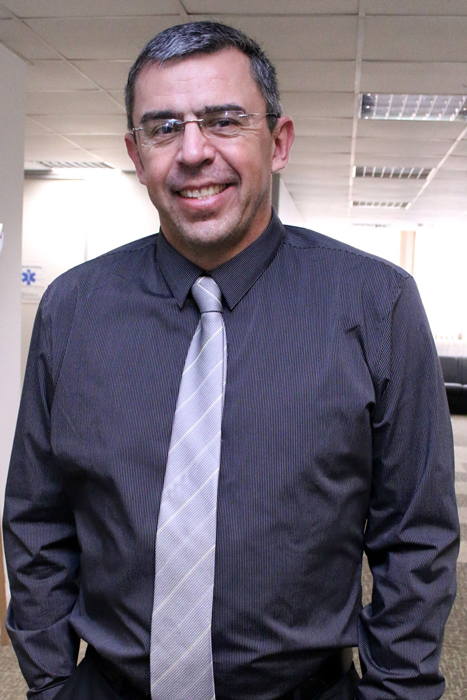
\includegraphics[width=0.8\textwidth]{pics/Rodacki}
\end{center}
\end{column}
\begin{column}{0.65\textwidth}
\begin{itemize}
\item<1-> Idealização e implementação.
\item<1-> Ampliação de temas e abrangência de público.
\item<1-> Superação.
\item<1-> Legado e inspiração.
\item<2-> Pessoal e institucionalmente: MUITO OBRIGADO.
\end{itemize}
\end{column}
\end{columns}
\end{frame}



\begin{frame}
  \frametitle{Equipe e agradecimentos - Instituições parceiras}
  Boas vindas à UFPR e agradecimentos adicionais.
  \\ \mbox{} \\
  Participantes de instituições públicas do Paraná.
  
  Representantes Institucionais
  \begin{itemize}
    \itemsep 1ex
  \item Stella Alonso Rocha, IFPR, Umuarama 
%  \item Rone B. Oliveira, UENP, 
  \item Airton Kist, UEPG, Ponta Grossa
  \item Jiam Frigo, Unila, Foz do Iguaçu
  \item Jerry Adriani Johann, Unioeste
%  \item Luciano Farinha Watzlawick, Unicentro
  \end{itemize}
 
\end{frame}


%% \begin{frame}[plain]
%%   \frametitle{Um elemento essencial}
%%   \begin{center}
%%     \LARGE{\textcolor{Magenta}{OS PARTICIPANTES}}
%%   \end{center}
  
%%   Onde voces estão?
%% \vspace{1cm}
%%   \begin{columns}
%% \begin{column}{0.75\textwidth}
%%     Acessar 
%%       \textit{\href{https://www.menti.com/7zs23636yf}{\bf este link}} (ou usar QRcode ao lado)\\
%%       e, no navegador, 
%%       digitar o nome da cidade onde está.
%% \end{column}
%% \begin{column}{0.25\textwidth}  %%<--- here
%%     \begin{center}
%%      \includegraphics[width=0.85\textwidth]{pics/QRCidades2021}
%%      \end{center}
%% \end{column}
%% \end{columns}
%% \end{frame}

\begin{frame}[plain]
  \frametitle{Participantes}

\begin{itemize}
\item PG's UFPR
\item PG's instituições parceiras
\item Professores
\item Outros
\end{itemize}

\vspace{0.5cm}
\pause
\LARGE{Onde voces estão?}

\vspace{0.5cm}

Acessar \\
\textit{\href{http://shiny.leg.ufpr.br/paulojus/cidades}{\bf http://shiny.leg.ufpr.br/paulojus/cidades}}\\
      e digitar o nome da cidade onde está.

\end{frame}


% --------------------------------------------

%\begin{frame}
%  \frametitle{Começando \ldots do começo}
%  \begin{center}
%    \Huge{\textcolor{Magenta}{Estatística?}}
%  \end{center}
%  
%  OK,  \\
%  estatística é \textit{importante} \ldots mas \ldots
%  \\
%  Que palavras/ideias \textbf{\it voce} associa com estatística?
%  \\
%  \vspace{0.5in}
%  Acesse \url[shiny.leg.ufpr.br/paulojus/estatistica]{este link}\\
%  e digite na interface ao menos cinco (5) palavras que voce associa com estatística.
%  
%\end{frame}

\begin{frame}[plain]
  \frametitle{Começando \ldots do começo}
  \begin{center}
    \LARGE{\textcolor{Magenta}{Estatística?}}
  \end{center}
   \frametitle{}
  OK, estatística é \textit{importante} \ldots mas \ldots
  \\
  Que palavras/ideias \textbf{\it voce} associa com estatística?
\vspace{1cm}

Acessar: \\
\textit{\href{http://shiny.leg.ufpr.br/paulojus/estatistica}{\bf http://shiny.leg.ufpr.br/paulojus/estatistica}}\\
e digite na interface até 3 termos (palavras-chave) que voce associa com estatística.

%% \begin{columns}
%% \begin{column}{0.75\textwidth}
%%     Acessar 
%%       \textit{\href{}{\bf }} \\% (ou usar QRcode ao lado)\\
%%       e digitar na interface três termos que voce associa com {\bf estatística}.
\begin{itemize}
   \item Apenas um termo (palavra chave) por linha.
   \item Usar apenas letras minúsculas.
   \item Evite plurais, procurar usar apenas termos no singular.
 \end{itemize}
%% \end{column}
%% \begin{column}{0.25\textwidth}  %%<--- here
%%     \begin{center}
%%      
\includegraphics[width=0.95\textwidth]{pics/QRestatistica}
%%      \end{center}
%% \end{column}
%% \end{columns}
\end{frame}

%--------------------------------------------


%% \begin{frame}
%% 	\frametitle{Resultados 2020}
%% 	\begin{center}
%% 	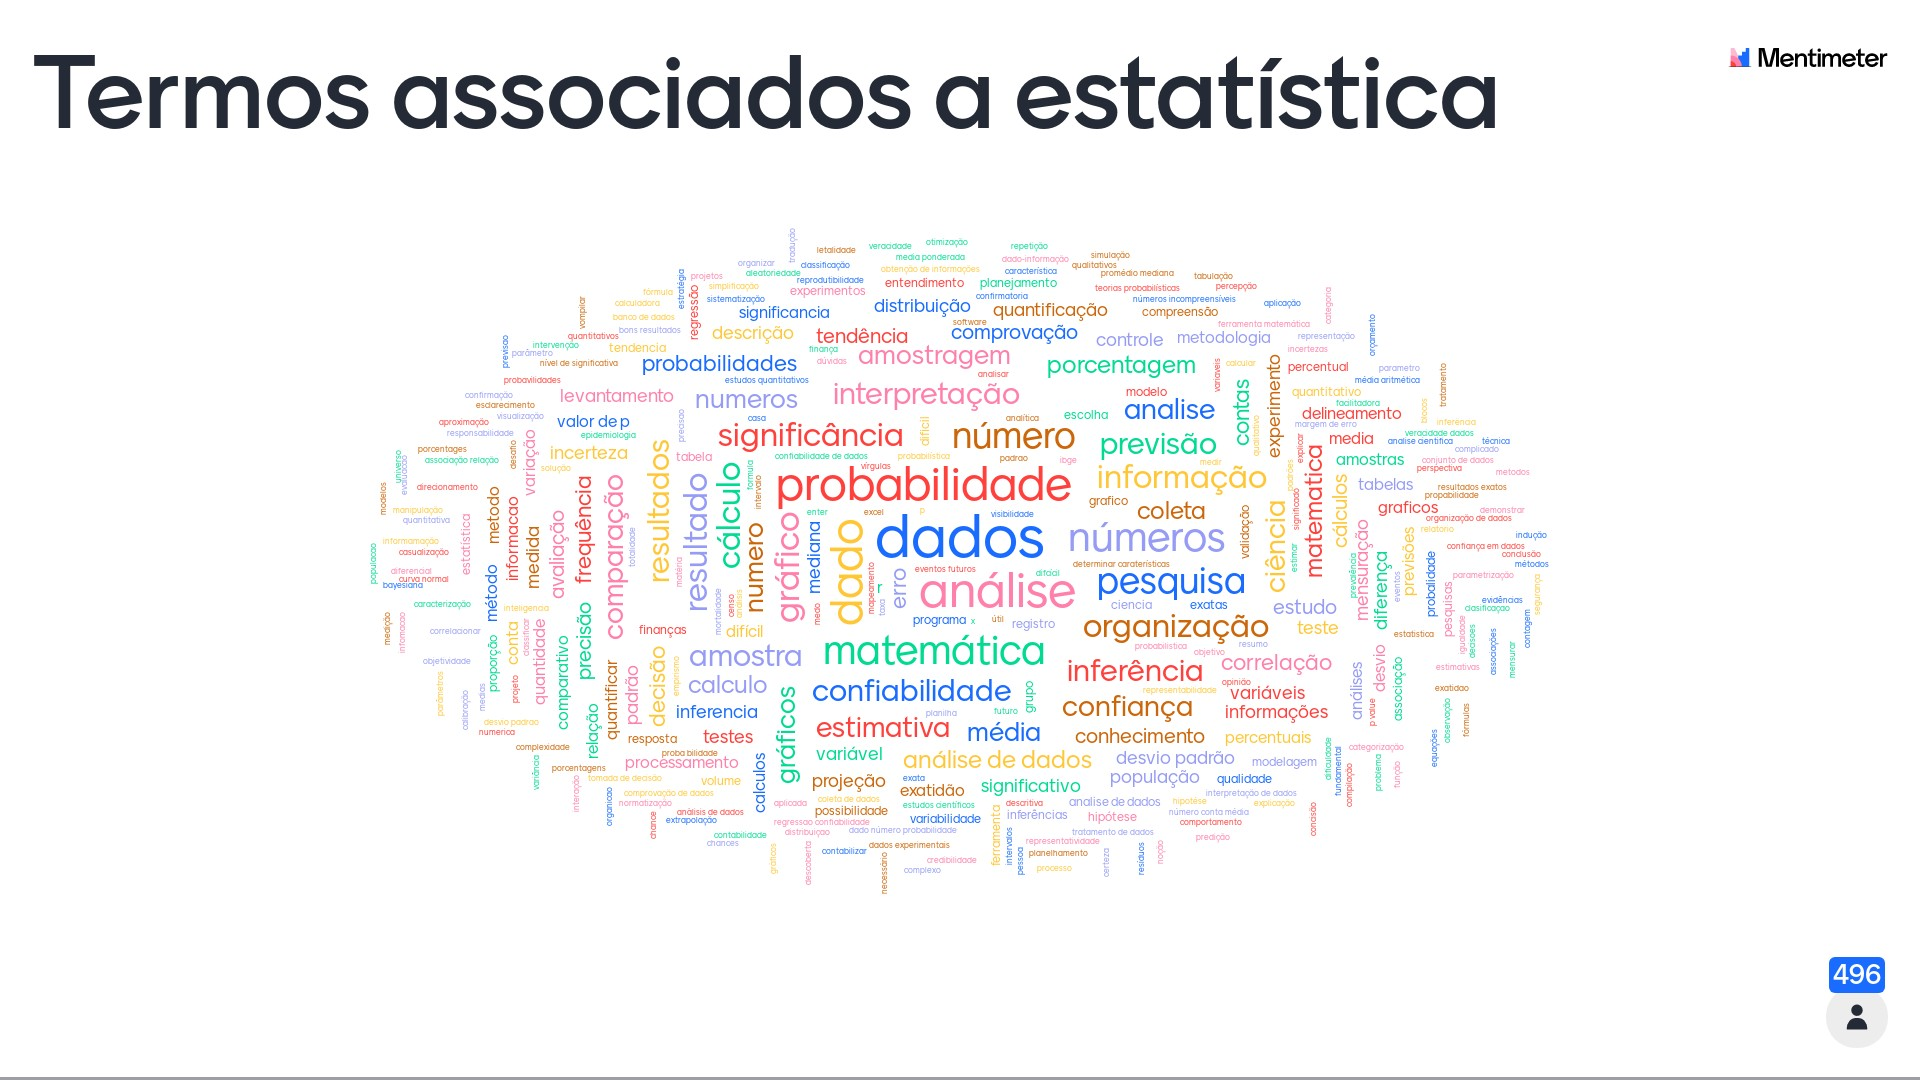
\includegraphics[height=0.95\textheight]{./pics/WC-Termos-2020}
%% \end{center}	

%% \end{frame}


\begin{frame}
  \frametitle{Temas nas respostas}

  Padrões? Recorrência?
  
  \pause
  
  \begin{itemize}
    \itemsep 2ex
  \item Dados I : obtenção, amostragem, pesquisa, volume, \ldots 
  \item Dados II: descrição, resumos, gráficos, análises, \ldots
  \item Probabilidades.
  \item Inferência: incerteza, população, amostra, testes, intervalos, \ldots
  \item Modelagem e métodos.
  \item \pause {\bf Interpretação.}
  \end{itemize}
  
\end{frame}


  
\begin{frame}
  \frametitle{Técnicas {\it vs} ideias: o propósito do curso}
  
\begin{figure}
\centering
\begin{minipage}{.5\textwidth}
  \centering
  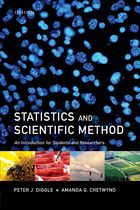
\includegraphics[width=0.55\textwidth]{./pics/diggle+chetwynd.jpg}
  \captionof{figure}{Diggle \& Chetwynd, 2011}
  \label{fig:diggle+chetwynd}
\end{minipage}%
\begin{minipage}{.5\textwidth}
  \centering
  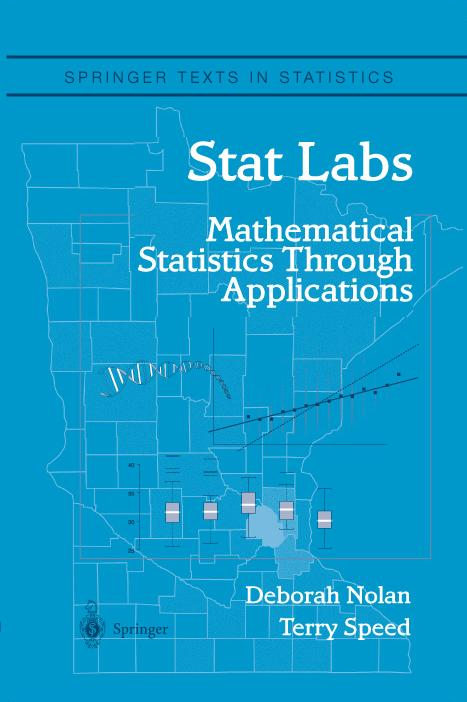
\includegraphics[width=0.55\textwidth]{./pics/statLabs.jpg}
  \captionof{figure}{Nolan \& Speed, 2000}
  \label{fig:nolan+speed}
\end{minipage}
\nocite{nolan+speed:2000,diggle+chetwynd:2011}
\end{figure}

\end{frame}

\begin{frame}
  \frametitle{Técnicas {\it vs} ideias: o propósito do curso}
  
  \begin{quote}
    More important than learning a few methods and techniques is to understand
    the {\it statistical thinking}.\\
    \hfill \cite{box+hunter+hunter:2005}
    % \hfill Box, Hunter \& Hunter \cite{box+hunter+hunter:2005}
  \end{quote}
  
  \pause
  
  \begin{itemize}
    \item Este \red{NÃO} é um curso orientado a técnicas. 
    \item Evitamos abordagem \textit{receita de bolo}. 
    \item Ênfase nos conceitos, no método estatístico, abordagens e paradigmas. 
    \item Exemplos motivam a exposição e discussões das ideias centrais.
    \item Análise crítica e interpretações no contexto de exemplos e métodos.
  \end{itemize}
  \pause
  \textit{Globo repórter da estatística !!??}
\end{frame}

%------------------------------------------------------------

\begin{frame}
  \frametitle{Um contexto: história e estatística}

\begin{figure}
    \centering
    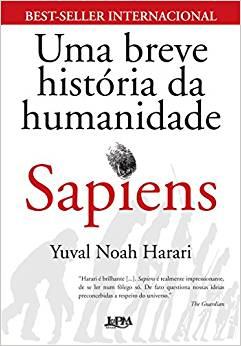
\includegraphics[width=.3\linewidth]{./pics/sapiens.jpeg}
    \caption{Harari, 2018}
\nocite{harari}
\end{figure}

\end{frame}


\begin{frame}
  \frametitle{Um contexto: história e estatística}

  Organização do Livro
  \begin{description}
    \itemsep 1.5ex
  \item Revolução cognitiva.
  \item Revolução agrícola.
  \item Unificação da humanidade.
  \item Revolução científica:
    \begin{itemize}
    \item a ``descoberta'' da ignorância (\textit{incerteza}).
    \end{itemize}
  \end{description}
\vspace{0.6cm}

Ciência moderna (em contraste tradições anteriores de conhecimento):
\begin{description}
\item disposição para admitir ignorância,
\item lugar central das observações e matemática,
\item aquisição de novas capacidades.
 \end{description} 

\end{frame}


\begin{frame}
  \frametitle{Um contexto: história e estatística }
  
  \begin{itemize}
    \itemsep 1.5ex
  \item \textit{\bf Ignoramus}
    \begin{itemize}
    \item  \textit{A Revolução Científica não foi uma revolução do conhecimento. \\
      Foi, acima de tudo uma revolução da ignorância}
    \end{itemize}
  \item \textit{\bf O dogma científico}
    \begin{itemize}
    \item  \textit{A ciência moderna não tem dogmas. Tem um conjunto da métodos de pesquisa em comum, todoas baseados em coletar observações empíricas e reuni-las com ajuda de ferramentas matemáticas.}
    \item \textit{Quando as observações atuais se chocam com tradições passadas, damos precedência às observações.}
    \item \textit{Aspiração de reduzir \ldots a equações \ldots inútil dada a complexidade \ldots} 
    \item \textit{Desenvolvimento de novo ramo \ldots {\bf estatística}.}
    \item \textit{Modelos probabilísticos (similares) se tornaram centrais em diversas áreas da ciência.}
    \item \textit{Há um movimento irresistível rumo às exatas \ldots em muitas áreas primeiro é preciso estudar estatística.}
    \end{itemize}
  \end{itemize}
\end{frame}

%--------------------------------------------------
\begin{frame}
  \frametitle{Uma possível definição}
  \begin{quote}
    Statistics is the \red{\it science} of collecting and interpreting data. \\
    \ldots\\
    Dealing with uncertainty is the cornerstone of the statistical method.\\
        \hfill \cite{diggle+chetwynd:2011}
  \end{quote}
\pause
  \begin{itemize}
    \itemsep 2ex
  \item Relevante em praticamente todas áreas do conhecimento.
  \item Dados e geral envolvem imprecisão e incerteza.
  \item Métodos: matemático (dedutivo) {\it vs} estatístico (inferêncial).
  \end{itemize}
\end{frame}

\begin{frame}
\frametitle{A necessidade de estatística}

\begin{itemize}
\item Dois pontos determinam uma reta! \ldots mesmo?
\item E se adicionarmos um terceiro? 
\item No mundo real pode não seguir padrão: imprevisibilidade ou erro?
\item \red{Erro} ou \red{desvio}? 
\item A natureza do \red{erro}
\item Se não podemos  ter certeza da reta, podemos ao menos estimar!
\end{itemize}

\end{frame}

\begin{frame}[fragile]
\frametitle{Estatística e o método científico}

\textit{Os dois pilares do método científico (para compreender a natureza) são:\\ {\bf teoria} e {\bf observação}.}
\vspace{-1cm}
\begin{knitrout}
\definecolor{shadecolor}{rgb}{0.992, 0.965, 0.89}\color{fgcolor}\begin{figure}

{\centering 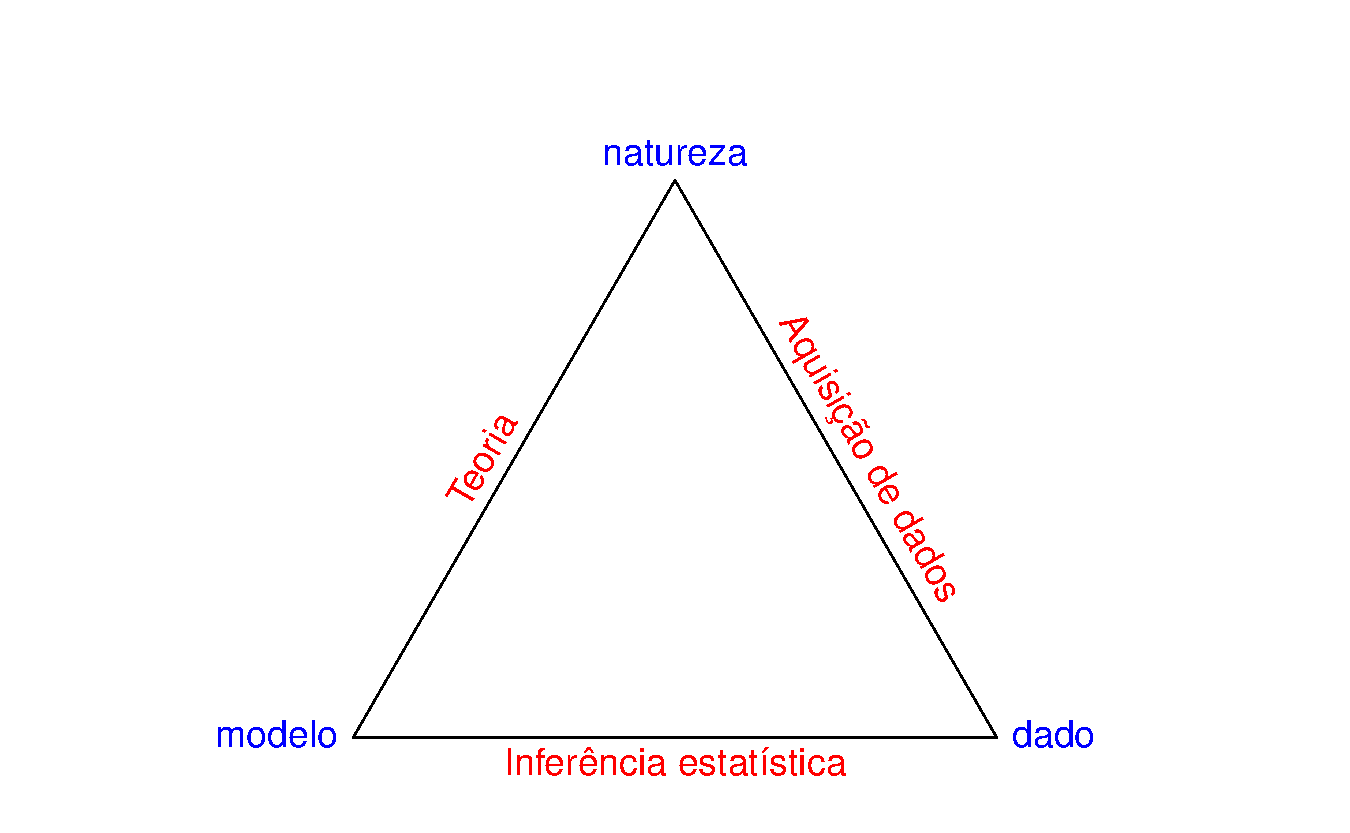
\includegraphics[width=11cm,height=0.75\textheight]{figure/unnamed-chunk-2-1} 

}

\caption{Estatística e o método científico (adaptado de \cite{diggle+chetwynd:2011}).}\label{fig:unnamed-chunk-2}
\end{figure}


\end{knitrout}
\end{frame}

\begin{frame}
  \frametitle{Estatística e o método científico}
\begin{knitrout}
\definecolor{shadecolor}{rgb}{0.992, 0.965, 0.89}\color{fgcolor}\begin{figure}

{\centering 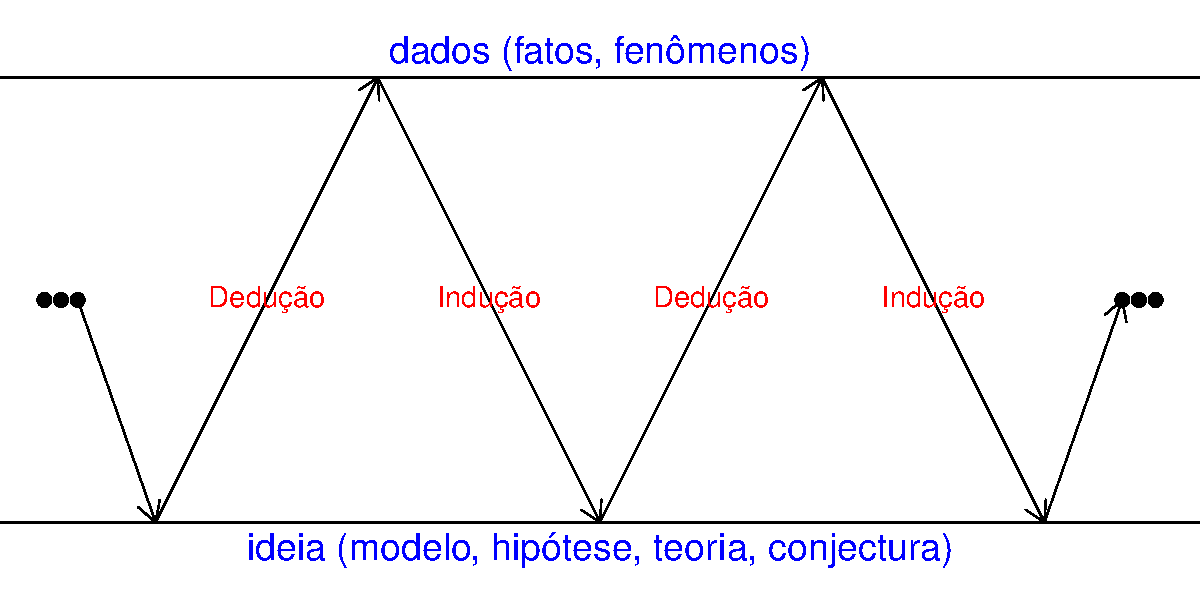
\includegraphics[width=11cm]{figure/unnamed-chunk-3-1} 

}

\caption{Processo do aprendizado (baseado em \cite{box+hunter+hunter:2005}).}\label{fig:unnamed-chunk-3}
\end{figure}


\end{knitrout}
\end{frame}

\begin{frame}
\frametitle{Princípios e ideias}
\begin{itemize}
\item Qual questão sobre a \blue{natureza} queremos investigar?
\item Pode ser \blue{respondida} por dados?
\item Qual \blue{experimento} possível pode fornecer os dados?
\item Como podemos \blue{aprender com os dados} sobre a questão de interesse?
\item Existe \red{incerteza}? Qual sua origem? Como mensurar?
\item Como \blue{avaliar} o que foi feito? 
\end{itemize}
\end{frame}


\begin{frame}
\frametitle{Mas, como a mágica acontece?}

Afinal, como na prática:
  \begin{itemize}
  \item se extrai informação dos dados,
  \item avalia-se  incerteza, 
  \item e orienta-se decisão utilizando métodos estatísticos?
  \end{itemize}
  \pause
  \textbf{Um exemplo (quase) trivial:}
\begin{itemize}
\item Considere uma população na qual deseja-se saber a proporção de indivíduos com certa característica.
\item Não sendo possível avaliar todos indivíduos, toma-se uma amostra.
\item Em 80 indivíduos amostrados, 19 mostram possuir o característica.
\item O que se pode concluir? Como expressar a incerteza? Como decidir se este valor supera uma proporção esperada de, digamos, 20\%?    
\end{itemize}  
\end{frame}

\begin{frame}
\frametitle{Como formalizar o "aprender com os dados"?}

\centering
\begin{figure}
  \centering
  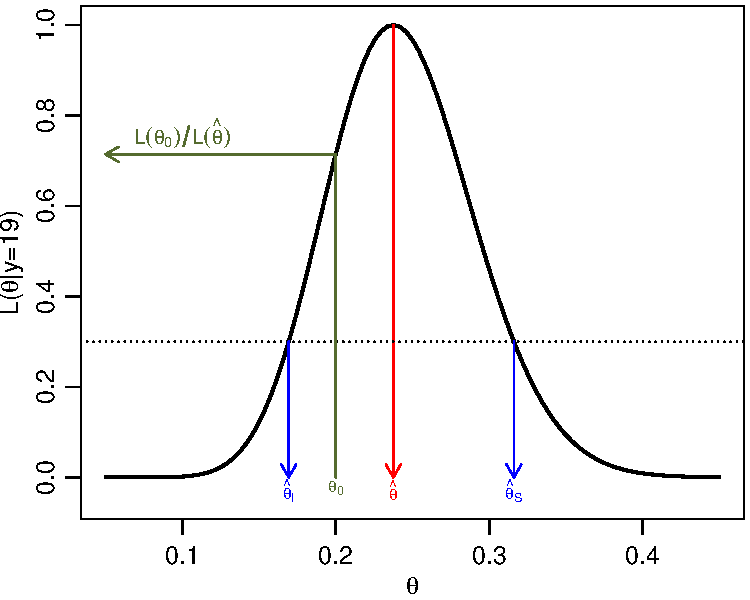
\includegraphics[height=0.45\textwidth]{pics/likelihood.pdf}
\caption{Uma função que expressa a informação dos dados.}
\end{figure}
\end{frame}


%% \begin{frame}
%% \frametitle{}

%% \begin{Huge}
%% Intervalo !!  \\
%% 15 minutos
%% \end{Huge}

%% Responder \textit{Quiz 1} disponível na página do Moodle

%% \end{frame}


%% \begin{frame}
%% \frametitle{Vamos conhecer a turma?}  

%% \pause

%% Tá bom então \ldots a apresentação fica por minha conta!\\

%% \vspace{2cm}

%% Vamos ao questionário! 

%% \end{frame}


%% \begin{frame}
%% \frametitle{Vamos conhecer a turma?}  

%% A ferramentas fornece um recurso de análise gráfica,\\ 
%% mas não é exatamento o que queremos \ldots \\

%% \vspace{1cm}
%% Queremos alterar e/ou adicionar gráficos

%% \vspace{1cm}
%% Queremos investigar relações entre respostas de diferentes questões

%% \end{frame}


%% \begin{frame}
%% \frametitle{}

%% \begin{Huge}
%% Mini-intervalo !!  \\
%% 5 minutos
%% \end{Huge}

%% Responder \textit{Quiz 2} disponível na página do Moodle
%% \\ \mbox{}\\
%% \ldots e retornamos com 
%% \red{\it \href{http://www.leg.ufpr.br/~paulojus/mepc2020/quest2020.html}{uma análise mais detalhada do questionário}}

%% \end{frame}


%% \begin{frame}
%%   \frametitle{Alguma análise}
%%   \itemsep 1ex
  
%%   \begin{itemize}
%%     \itemsep 1.5ex
%%   \item O objetivo da análise: descrição do perfil? \pause
%%   \item População ou amostra? 
%%     \begin{itemize}
%%     \item (de) qual população? \pause
%%     \end{itemize}
%% %  \item Que gráficos (ou análises) fazer? 
%% %  \item Gráficos/análises: uni, bi e multivariadas
%% %  \item Tipos de variáveis
%% %    \begin{itemize}
%% %    \item qualitativas (nominais ou ordinais)
%% %    \item quantitativas (discretas ou contínuas)
%% %    \end{itemize}
%%   \end{itemize}
%% \end{frame}

%% \begin{frame}
%%   \frametitle{As dificuldades aparecem \ldots}
%%   \begin{itemize}
%%     \itemsep 1.5ex
%%   \item (pré) validação do questionário
%%   \item respostas inesperadas
%%   \item questões para checagem de coerência
%%   \item desenho das questões e alternativas
%%   \item tratamento (automático) de anomalias
%%   \item processamento (automático) e adequação de respostas em texto
%%   \item descarte (questão ou questionário)
%%   \item \ldots
%%   \end{itemize}
%%   \textit{Pagar na entrada ou na saída?}
%% \end{frame}

%% \begin{frame}
%%   \frametitle{Removidas as dificuldades \ldots}
%%   \itemsep 1ex
  
%%   \begin{itemize}
%%     \itemsep 1.5ex
%%   \item Que gráficos (ou análises) fazer? 
%%   \item Gráficos/análises: uni, bi e multivariadas
%%   \item Tipos de variáveis
%%     \begin{itemize}
%%     \item qualitativas (nominais ou ordinais)
%%     \item quantitativas (discretas ou contínuas)
%%     \end{itemize}
%%   \end{itemize}
%% \end{frame}


%% \begin{frame}
%%   \frametitle{De onde vêm os dados?}

%%   Fontes usuais:
%%   \begin{itemize}
%%     \itemsep 1.5ex
%%   \item questionários
%%   \item amostragens
%%   \item experimentos
%%   \item observacionais
%%   \item repositórios
%%   \item bancos de dados
%%   \item web (processamento)
%%   \item \ldots
%%   \end{itemize}

%% \pause

%% Questão fundamental e nem sempre trivial:\\
%% Qual universo os dados representam?

%% \end{frame}


\begin{frame}
\frametitle{Informações sobre o curso}
\textbf{Programa}
\begin{enumerate}
\item Fundamentos
  \begin{enumerate}
  \item Estatística descritiva/exploratória
  \item Probabilidades
  \item Princípios de inferência e paradigmas
  \end{enumerate}
\item Métodos, modelos e extras
  \begin{enumerate}
  \item Amostragem
  \item Visualização de dados
  \item Tópicos em estatística e computação
  \item Tópicos em aprendizado de máquina e {\it big data}
  \item Pesquisa reproduzível
  \item Regressão
  \item Extensões de regressão
%  \item Árvores de regressão e classificação 
  \item Dados Longitudinais
%  \item Métodos Multivariados
  \item Análise de sobrevivência
  \item Teoria de avaliação
  \item Análise de imagens
  \item Dados categóricos
  \end{enumerate}
\end{enumerate}

\end{frame}


\begin{frame}
  \frametitle{Textos de apoio - parte inicial}
\begin{figure}
\centering
\begin{minipage}{.5\textwidth}
  \centering
  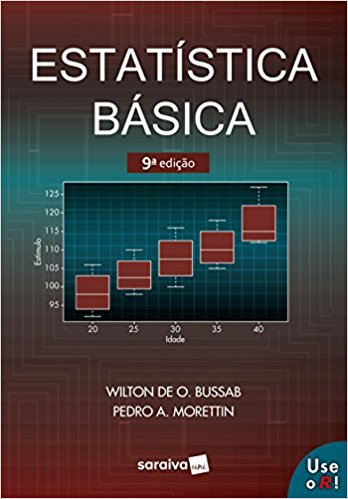
\includegraphics[width=0.55\textwidth]{./pics/BussabMorettin.jpg}
  \captionof{figure}{Bussab \& Morettin}
  \label{fig:bussab+morettin}
\end{minipage}%
\begin{minipage}{.5\textwidth}
  \centering
  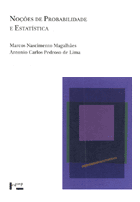
\includegraphics[width=0.55\textwidth]{./pics/noproest.png}
  \captionof{figure}{Magalhães \& Lima}
  \label{fig:magalhaes+lima}
\end{minipage}
\end{figure}
\nocite{bussab+morettin:2017,magalhaes+lima:2015}
\end{frame}


\begin{frame}
  \frametitle{Textos de apoio - parte inicial}
\begin{figure}
\centering
\begin{minipage}{.33\textwidth}
  \centering
  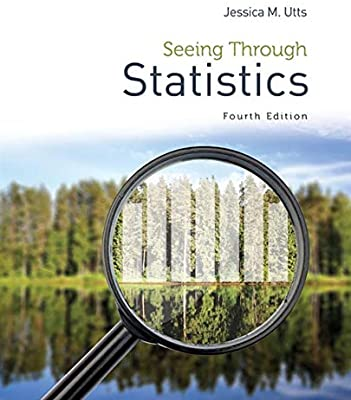
\includegraphics[width=0.8\textwidth]{./pics/SeeingStatistics.jpg}
  \captionof{figure}{Utts}
  \label{fig:utts}
\end{minipage}%
\begin{minipage}{.33\textwidth}
  \centering
  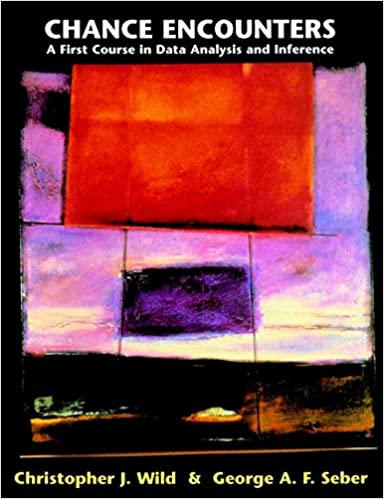
\includegraphics[width=0.8\textwidth]{./pics/ChanceEncounters.jpg}
  \captionof{figure}{Wild \& Seber}
  \label{fig:wild+seber}
\end{minipage}
\begin{minipage}{.33\textwidth}
  \centering
  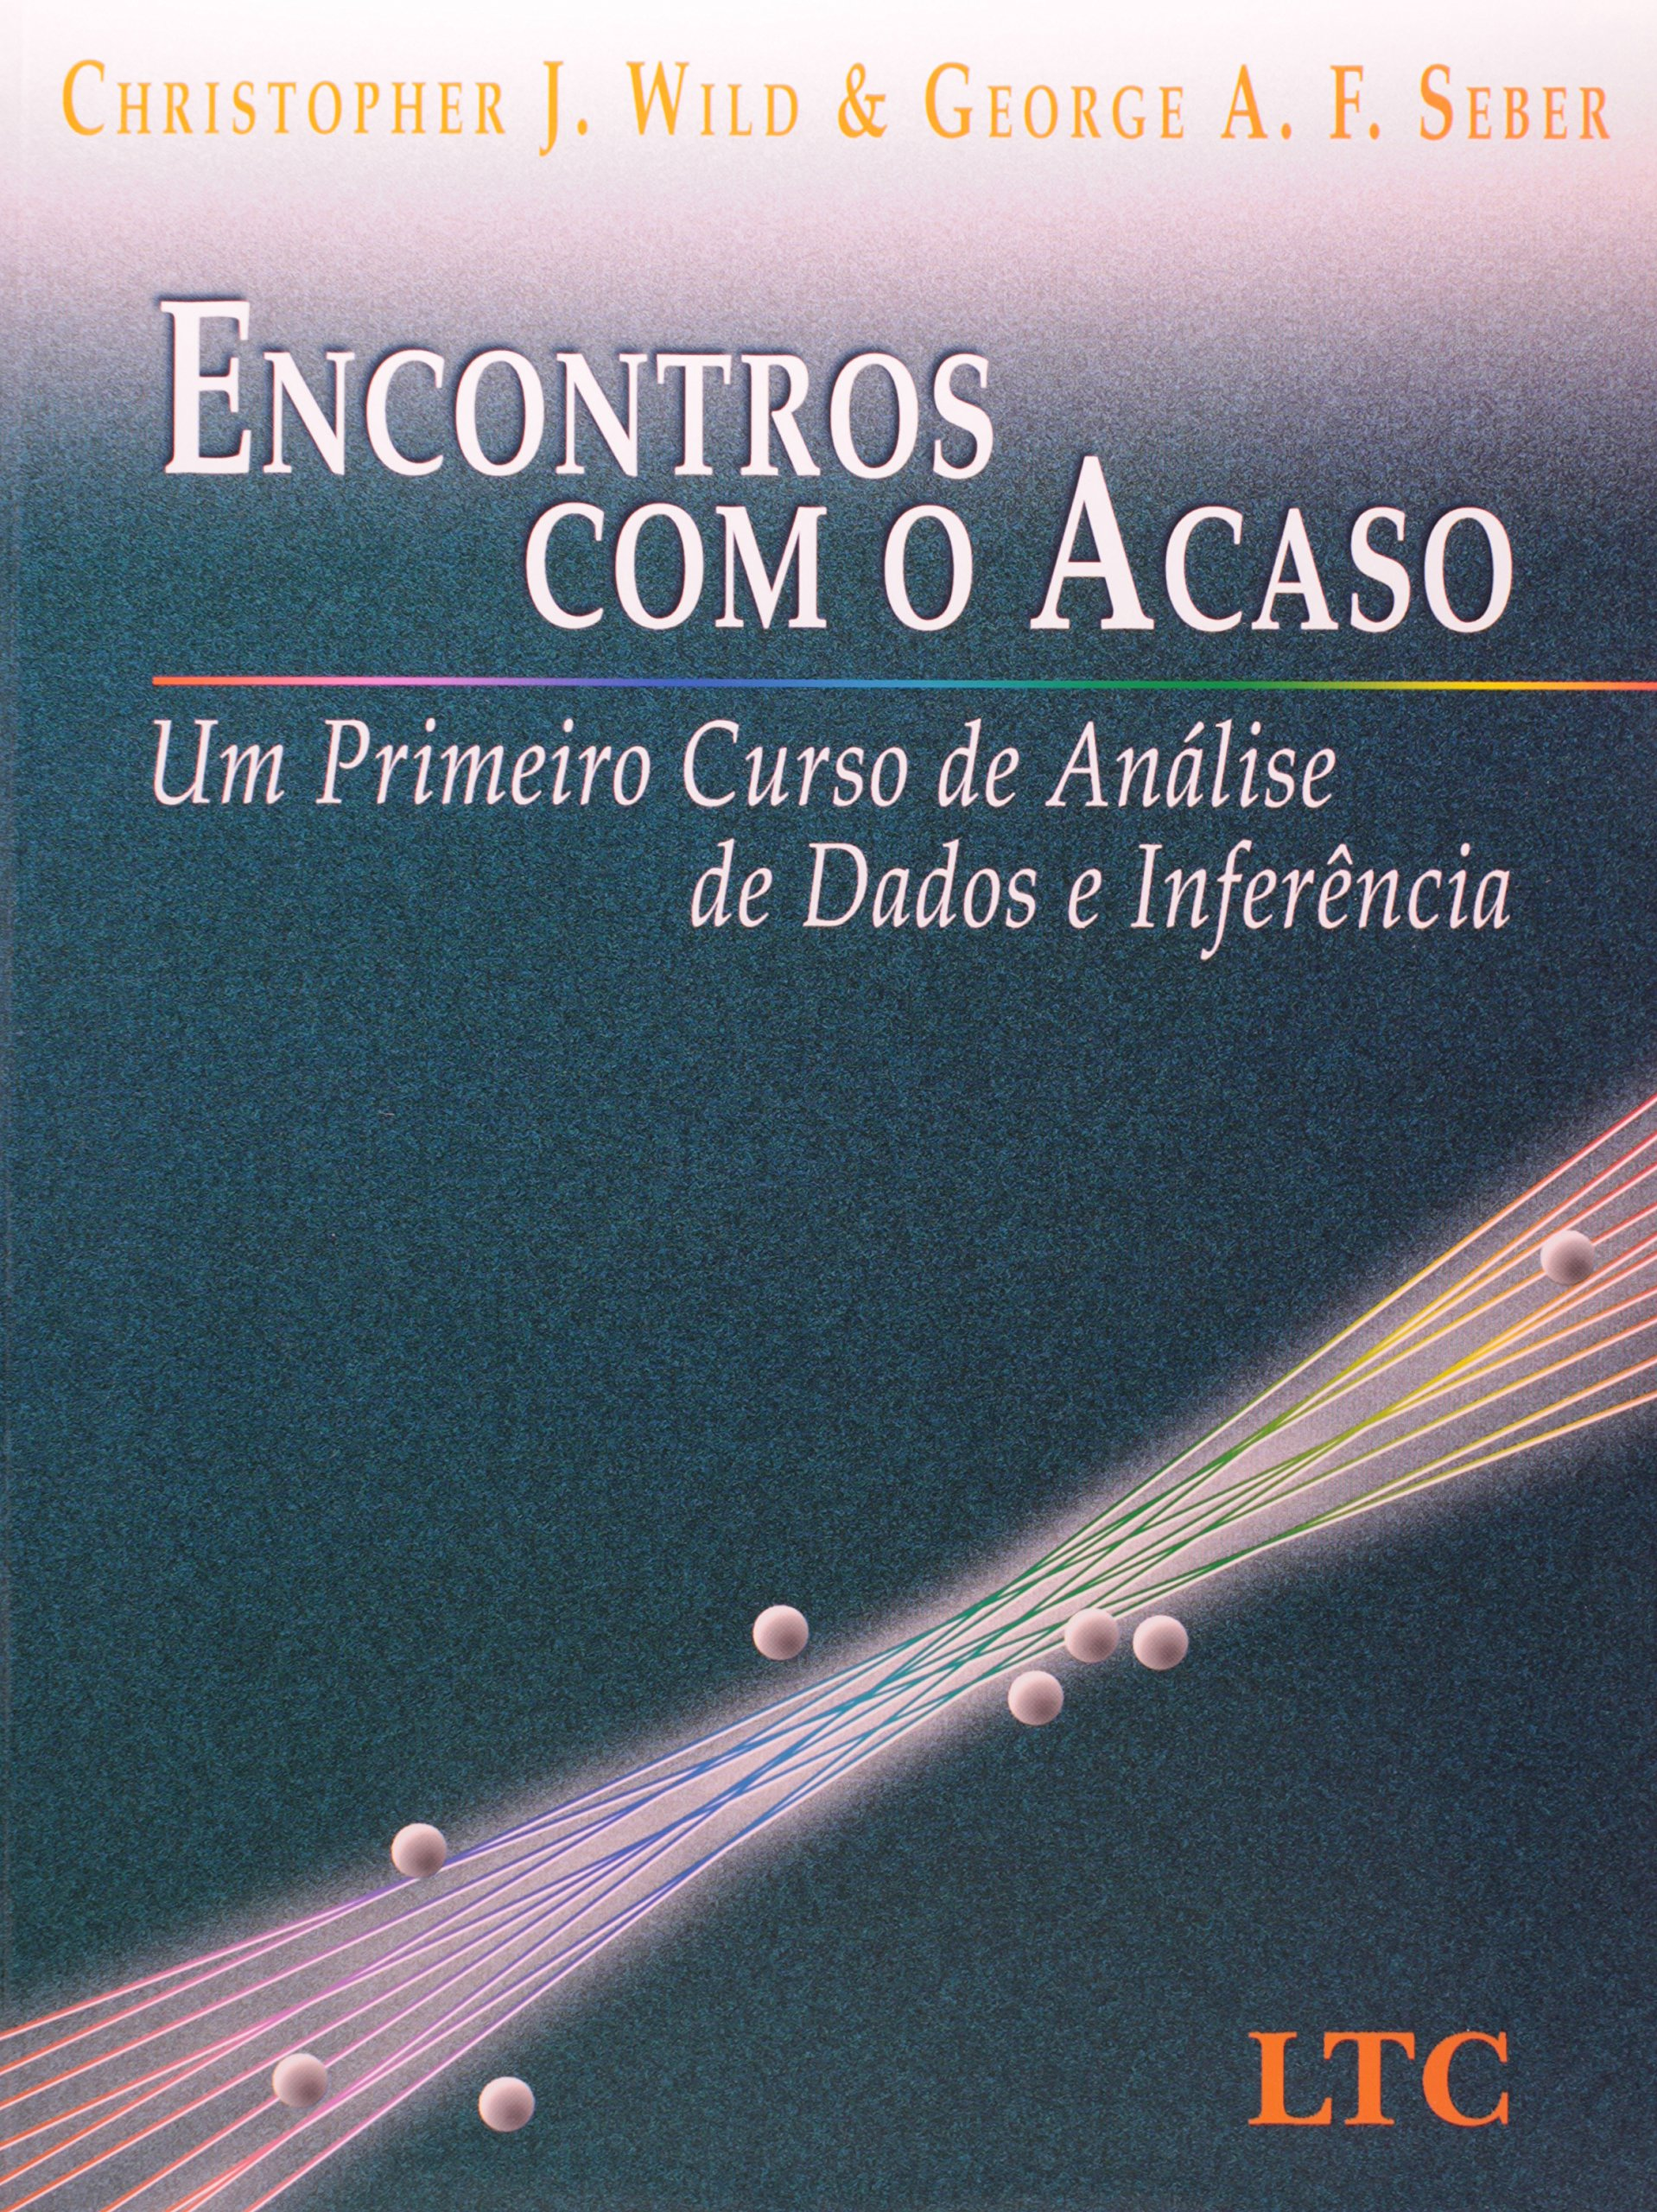
\includegraphics[width=0.8\textwidth]{./pics/EncontrosAcaso.jpg}
  \captionof{figure}{Wild \& Seber (PT)}
  \label{fig:wild+seber+pt}
\end{minipage}
\end{figure}
\nocite{wild+seber:2000,wild+seber:2004,utts:2005}
\end{frame}

% \begin{frame}
%  \frametitle{Textos de apoio}
%  \begin{figure}
%    \centering
%    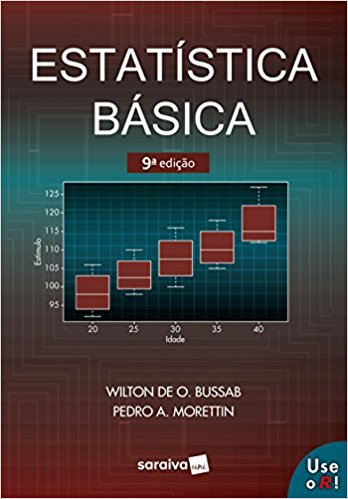
\includegraphics[width=.4\linewidth]{./pics/BussabMorettin.jpg}
%    % \includegraphics[width=.4\linewidth]{image1}
%  \caption{Bussab \& Morettin, 2017}
%  \end{figure}  
%\end{frame}


\begin{frame}
  \frametitle{Dinâmica}  
  \begin{itemize}
  \item Materiais pré-aula
  \item Enquete pré-aula.
  \item Aulas remotas (ao vivo) às quartas (15 semanas).
    \begin{itemize}
    \item Parte 1: antes do 1o intervalo: conceitual.
    \item Parte 2: após 1o intervalo: conceitual.
    \item Parte 3: após 2o intervalo: tópicos em \textsl{\bf R} (opcional).
    \item Controle de frequência online (durante as aulas - horários fixados).
    \item CHAT durante a aula, perguntas/comentários, via monitores.
    \end{itemize}
  \item Forum aberto para cada aula: forum geral, da semana e email.
  \item Disponibilização de material e atividades recomendadas pelo moodle.
  \item Disponibilização de vídeo da aula (link pelo moodle).
  \item Avaliação 
    \begin{itemize}
    \item participação nas atividades (enquetes, etc).
    \item \textit{quizzes} semanais via moodle.
    \item provas via moodle.
%    \item atividades relacionada à área (avaliação pelo orientador)
    \end{itemize}
\end{itemize}
\end{frame}

\begin{frame}
  \frametitle{Contatos}
  \textbf{Coordenação/administração:}
  \begin{itemize}
     \item Administrativa: matrículas, acesso ao sistema e similares: \\ Equipe das Transversais (\red{transversal@ufpr.br}) 
 \end{itemize}
  \textbf{Apoio acadêmico:}
  \begin{itemize}
  \item Acadêmica/conteúdo: monitores e professores \\ Equipe MEPC (\red{mepc2021@ufpr.br}).
  \end{itemize}

  
  \red{\bf Para organização, rastreamento e efetividade nas respostas:} \\
  NÃO enviar emails relacionados ao curso para endereços pessoais dos professores e monitores do curso.
\end{frame}



\begin{frame}[fragile]
  \frametitle{Referências bibliográficas}
  
  \begin{tiny}
    \bibliography{references}
  \end{tiny}
  
\end{frame}


\end{document}
